\documentclass[aspectratio=169,17pt]{beamer}
\usepackage{ulem}

\usepackage{../theme/polygl0ts}

% warns about obsolete commands
\usepackage{nag}

% fractions
\usepackage{xfrac}

%% Font preferences
%\usepackage[oldstyle,semibold]{libertinus} % not good on black bg
\usepackage[oldstyle,semibold]{noto}

% self-explanatory
\usepackage{qrcode}

%\setbeameroption{show notes on second screen}

\tikzstyle{freecell}=[fill=none]

\newcommand{\reg}[1]{\%\mintinline{asm}{#1}}
\newcommand{\hex}[1]{\mintinline{python}{0x#1}}
\newcommand{\naddr}[2]{\begin{tabular}{l}#1\\\hex{#2}\end{tabular}}
\newcommand{\docl}[1]{(\textbf{\href{#1}{Documentation}})}


%% Proper 1337 typography
\newcommand\SlashedZero{{%
\addfontfeatures{RawFeature=+zero}%
\addfontfeatures{RawFeature=-pnum}%
\addfontfeatures{RawFeature=-onum}%
0%
}}
\newcommand\organizers{\SlashedZero{}rganizers}
\newcommand\polyglots{polygl\SlashedZero{}ts}

\newcommand\biglink[1]{
	\begin{center}
		\colorbox{white}{
		\textcolor{black}{
		\qrcode*[height=.8\textheight]{#1}
	}
	}

		\url{#1}
	\end{center}
}

\hypersetup{colorlinks,linkcolor=,urlcolor=brightblue}

\setbeamertemplate{navigation symbols}{}

\setbeameroption{show notes}

\showsectionframe{}

%%%%%%%%%%%%%%%%%%%%%%%%%%%%%%%%%%%%%%%%%%%%%%%%%%%%%%%%%%%%%%%%%%%%%%%%%%%%%%%
% Title Setup
%%%%%%%%%%%%%%%%%%%%%%%%%%%%%%%%%%%%%%%%%%%%%%%%%%%%%%%%%%%%%%%%%%%%%%%%%%%%%%%
\title{Web3 CTF}
\author{\texttt{0xbbjubjub}}
\institute{\polyglots}
\date{8 November 2024}
\begin{document}
\titleframe{}

\section{A History Lesson}
\begin{frame}
	\centering
	
\includegraphics[height=.7\textheight]{assets/1200px-Bitcoin.svg.png}

	In the beginning Crypto 
\includegraphics[width=1em]{assets/psyduck.png} made Bitcoin
\end{frame}

\begin{frame}
	\begin{description}
		\item[Goal] be an immaterial asset with no central server
		\item[Problem] keep track of balances
		\item[Solution] a public database with no administrator
	\end{description}
\end{frame}

\begin{frame}
	\frametitle{The Bitcoin Database Schema (simplified!)}
	\begin{tabular}{ccl}
		\ttfamily amount & \ttfamily integer & amount of bitcoin
		\\
		\ttfamily owner & \ttfamily bytes20 & owner public key
		\\
		\ttfamily spent & \ttfamily boolean & if the bitcoin has been spent
	\end{tabular}
\end{frame}

\begin{frame}
	\frametitle{Bitcoin Transaction Rules}
	\begin{itemize}
		\item must be cryptographically \emph{signed} by owners
			\pause{}
		\item can spend bitcoin that's \emph{unspent}
			\pause{}
		\item can only spend owners' \emph{own} bitcoin
			\pause{}
		\item can create new unspent rows in the database
			\pause{}
		\item can assign as much bitcoin as it spends
	\end{itemize}
\end{frame}

\begin{frame}
	\frametitle{Choosing Transactions}
	Bitcoin assigns the right to choose the next transactions via \emph{lottery}.

	This is a proof-of-work lottery: the first to find a hash starting with n zeroes win.
\end{frame}

\begin{frame}
	The chosen \emph{miner} publishes a block: a list of transactions + the hash of the previous block.

	This forms a \emph{blockchain}: an append-only log of all the transactions that ever took place.
\end{frame}
\begin{frame}
	\frametitle{Putting Bitcoin Together}

	Proof-of-work achieves \emph{consensus}: everyone follows the chain with the most proof-of-work and sees the same state.

	The \emph{rules} inside the replicated database are \emph{hard-coded}.
	We have one application: bitcoin transfer.
\end{frame}

\begin{frame}
	\frametitle{Tweaking Bitcoin}

	\centering
	
\includegraphics[width=.4\textwidth]{assets/monero-symbol-on-white-1280.png}
	
\includegraphics[width=.4\textwidth]{assets/namecoin.png}
\end{frame}

\begin{frame}
	\frametitle{Limitations}
	Need to build own P2P network and miner base \emph{from scratch}

	Cannot \emph{interoperate} easily with Bitcoin
\end{frame}

\begin{frame}
	\frametitle{Smart Contracts}
	Database rules should be more \emph{general}

	People can make their own tables

	Allow executing arbitrary logic
\end{frame}

\begin{frame}
	\frametitle{Ethereum}
	\centering
	
\includegraphics[height=.9\textheight]{assets/Eth-diamond-rainbow.png}
\end{frame}

\begin{frame}
	\centering
	Code has Bugs!
\end{frame}

\begin{frame}
	\centering
	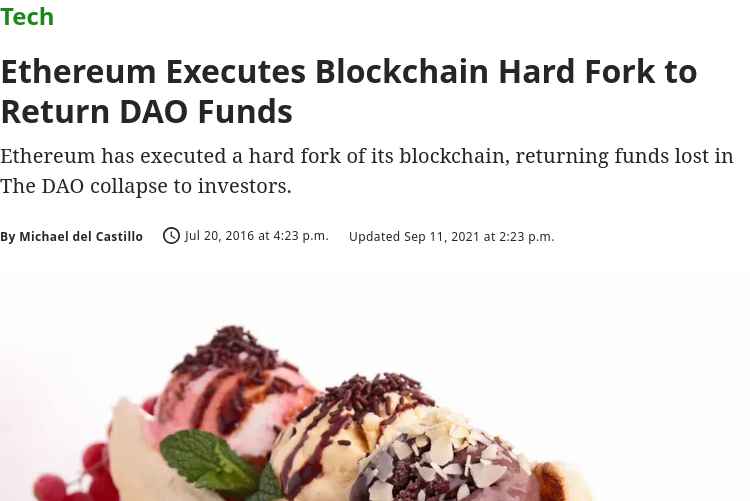
\includegraphics[height=.9\textheight]{assets/daofork.png}
\end{frame}

\begin{frame}
	\centering
	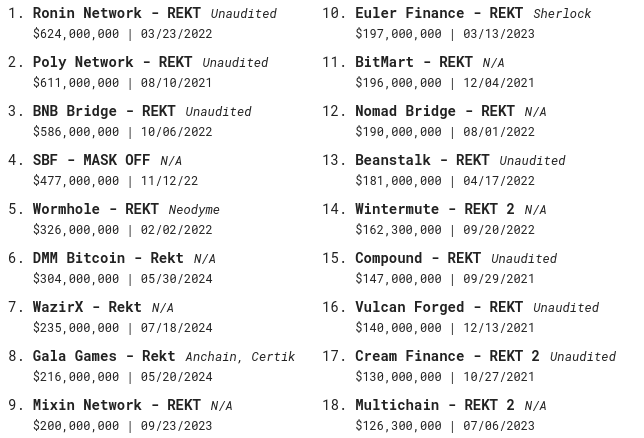
\includegraphics[height=.9\textheight]{assets/rekt.png}
\end{frame}

\begin{frame}
	Get on the Internet and send out a major distress signal
\end{frame}

\begin{frame}
	\frametitle{Web3 Security}
	``Hackers will look at my code anyway, it needs to be ones I'm paying!''
\end{frame}

\begin{frame}
	\begin{itemize}
		\item Code auditing
		\item Bug bounty
		\item Incident response
	\end{itemize}
\end{frame}

	\section{Your Target}
\begin{frame}
	\frametitle{Ethereum Virtual Machine}
	Stack-based VM, 256-bit(!), metered
	\pause{}
	\url{evm.codes}
\end{frame}

\begin{frame}
	\frametitle{Smart Contracts}
	Deploy your EVM bytecode, people and other contracts can call it at will.
\end{frame}

\begin{frame}
	\frametitle{Input/Output}
	\emph{calldata}: message from whoever called
	\emph{returndata}: the dual of calldata
\end{frame}

\begin{frame}
	\frametitle{Volatile memory}
	\begin{description}
		\item[Stack] 1024 256-bit slots
		\item[Memory] byte-addressed, contiguous
	\end{description}
\end{frame}

\begin{frame}
	\frametitle{Persistent Memory}
	$2^{256}$ 256-bit slots per smart contract

	Using a new slot cost \emph{a lot} of gas
\end{frame}

\begin{frame}
	\frametitle{Keccak256}
	\emph{cryptographic hash function}
	that EVM has \emph{built-in} access to
\end{frame}

\begin{frame}
	\frametitle{Mapping Pattern}
	To store key-value pairs:

	\begin{enumerate}
		\item serialize and hash the key in-context
		\item convert the hash to unsigned integer
		\item store the key at the numbered slot
	\end{enumerate}
\end{frame}

\begin{frame}
	\frametitle{Atomicity}
	\emph{Transactional} database: failure cancels changes

	%\texttt{REVERT} undoes any changes, unwinds the stack, but can be recovered from
\end{frame}

\begin{frame}
	\begin{center}
		\biglink{https://discord.gg/VEtQUytz}
	\end{center}
\end{frame}
\end{document}
